\documentclass{article}

% 字体设置
\usepackage[no-math]{fontspec}
\setmainfont{Times New Roman}
\usepackage[UTF8]{ctex}
% \setCJKmainfont{Noto Serif SC}[ItalicFont=方正仿宋_GBK]
% \setCJKmathfont{Noto Serif SC}[ItalicFont=方正仿宋_GBK]

% 数学输入
\usepackage{amsmath}
\usepackage{amsfonts}
\usepackage{amssymb}
\usepackage{esint}
\usepackage{tikz}
\usepackage{latexsym}

% 排版设置
\usepackage{enumitem}
\usepackage{xcolor}
\usepackage{geometry}
% \geometry{a5paper}
% \geometry{left=0.3cm, right=0.3cm, top=1.7cm, bottom=1.7cm}
\geometry{a4paper}
\geometry{left=1.9cm, right=1.9cm, top=1.7cm, bottom=1.7cm}

% 表格
\usepackage{array}
\usepackage{tabularx}
\usepackage{caption}
\providecommand{\tightlist}{\setlength{\itemsep}{0pt}\setlength{\parskip}{0pt}}
\usepackage{siunitx}

% 超链接
\usepackage{hyperref}
\urlstyle{rm}
\hypersetup{
    colorlinks=true, 
    linkcolor=black, 
    citecolor=black, 
    urlcolor=black, 
    bookmarks=true, 
    bookmarksopen=true, 
    bookmarksnumbered=true, 
}

% 标题和作者设置
\title{实验 1 \ \ 熟悉 Vivado 环境}
\author{Chen-Yuanmeng \thanks{Email: \url{chenyumeng23@mails.ucas.ac.cn}}}
\date{2024/10/17}

% 定义代码环境
\usepackage{listings}

\definecolor{codegreen}{rgb}{0, 0.6, 0}
\definecolor{codegray}{rgb}{0.5, 0.5, 0.5}
\definecolor{codepurple}{rgb}{0.58, 0, 0.82}
\definecolor{backcolour}{rgb}{0.95, 0.95, 0.92}

\definecolor{dkgreen}{rgb}{0,0.6,0}
\definecolor{gray}{rgb}{0.5,0.5,0.5}
\definecolor{mauve}{rgb}{0.58,0,0.82}
\lstset{
  frame=tb,
  aboveskip=3mm,
  belowskip=3mm,
  showstringspaces=false,
  columns=flexible,
  framerule=1pt,
  rulecolor=\color{gray!35},
  backgroundcolor=\color{gray!5},
  basicstyle={\small\ttfamily},
  numbers=none,
  numberstyle=\tiny\color{gray},
  keywordstyle=\color{blue},
  commentstyle=\color{dkgreen},
  stringstyle=\color{mauve},
  breaklines=true,
  breakatwhitespace=true,
  tabsize=3,
  language=Verilog
}

\begin{document}

\maketitle

\section{实验目的}

\begin{enumerate}\tightlist
    \item 熟悉 Vivado 设计流程
    \item 掌握利用 Vivado 创建设计的方法(以实现4位加法器为例)
    \item 熟练 Verilog 语法
    \item 掌握编写 Testbench 的方法,以及行为仿真方法
\end{enumerate}

\section{实验环境}

\begin{itemize}\tightlist
    \item Microsoft Windows 10.0.19043.928
    \item Vivado v2017.4 (64-bit)
    \item 玉泉路一机房
\end{itemize}

\section{原理说明}

\subsection{4位加法器}

直接使用计算功能进行计算即可, 代码如下:
\begin{lstlisting}
    assign {c_out, out} = add_0 + add_1 + c_in;
\end{lstlisting}

\subsection{全加器 (门电路版本)}

根据全加器的定义, 知道 \(S = A \oplus B \oplus C_i\), \(C_o = AB + AC_i + BC_i\). 据此写出 Verilog 代码即可:
\begin{lstlisting}
    assign s = (a ^ b) ^ ci;
    assign co = (a & b) | (a & ci) | (b & ci);
\end{lstlisting}

\subsection{3--8译码器 (高电平有效)}

在控制序列的三位分别为 \lstinline|3'b100| 的时候, 将输入的3位二进制数转化为相应的一个电平信号输出, 可以用 \lstinline|case| 语句. 控制语句可用 \lstinline|if| 判断. 具体如下:
\begin{lstlisting}
    always @(*) begin
        case(a)
            3'b000: out = 8'b1;
            3'b001: out = 8'b10;
            3'b010: out = 8'b100;
            3'b011: out = 8'b1000;
            3'b100: out = 8'b10000;
            3'b101: out = 8'b100000;
            3'b110: out = 8'b1000000;
            3'b111: out = 8'b10000000;
        endcase
        
        if (cs != 3'b110) begin
            out= 8'b0;
        end
    end
\end{lstlisting}

\section{接口定义}

\subsection{4位加法器}

\begin{lstlisting}
    input [3:0] add_0,      \\ 加数 1
    input [3:0] add_1,      \\ 加数 2
    input c_in,             \\ 进位输入
    output [3:0] out,       \\ 输出
    output c_out            \\ 进位输出
\end{lstlisting}

\subsection{全加器 (门电路版本)}

\begin{lstlisting}
    input a,    \\ 加数 1
    input b,    \\ 加数 2
    input ci,   \\ 进位输入
    output s,   \\ 本位输出
    output co   \\ 进位输出
\end{lstlisting}

\subsection{3--8译码器 (高电平有效)}

\begin{lstlisting}
    input [2:0] a,      \\ 输入的 3 位二进制数码
    input [2:0] cs,     \\ 控制序列 (当且仅当为 110 时, 有效输出)
    output [7:0] y      \\ 输出的 8 位电平
\end{lstlisting}

\section{调试过程及结果}

点击左侧 ``SIMULATION'' 下的 ``Run Simulation'', 以默认设置进行模拟调试. 调试结果分别如图所示:

\subsection{4位加法器}

\begin{center}
    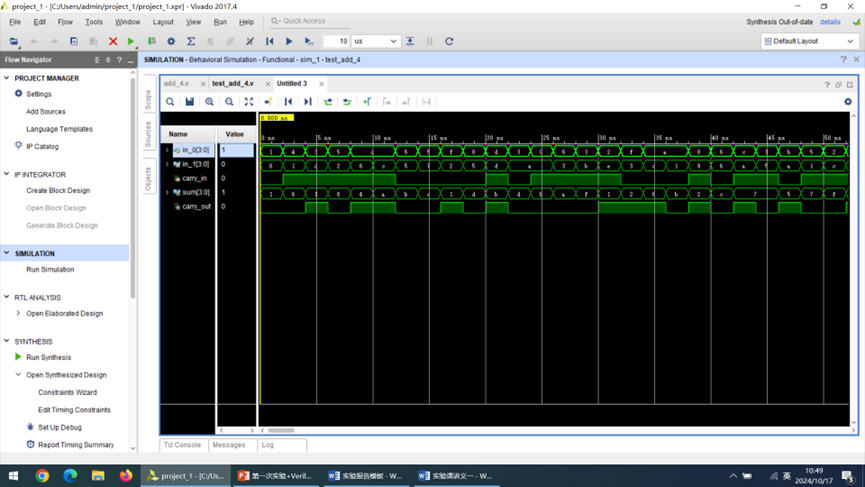
\includegraphics{assets/image_4_adder.png}
    \captionof{figure}{4位加法器 Simulation 结果}
\end{center}

\subsection{全加器 (门电路版本)}

\begin{center}
    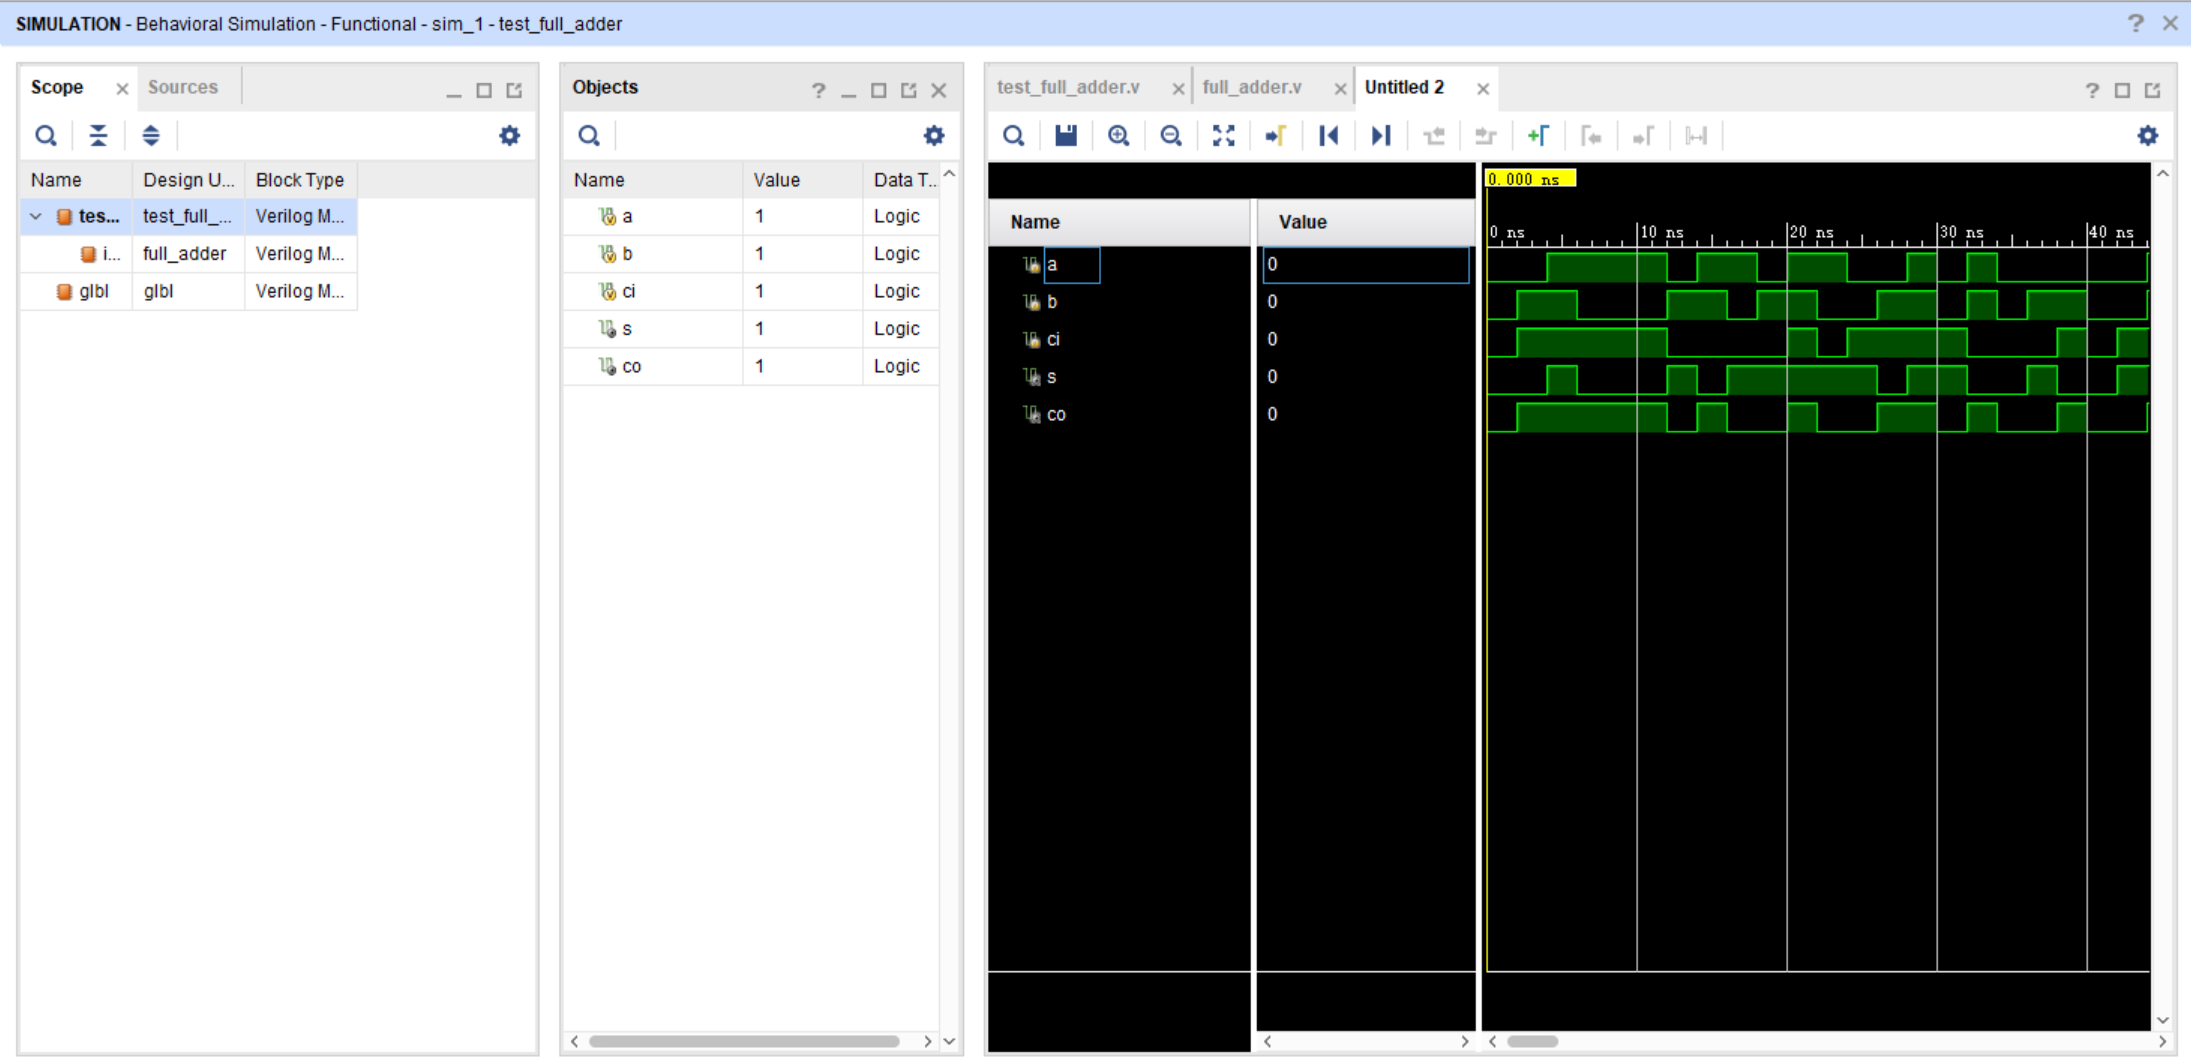
\includegraphics[width=500pt]{assets/image_full_adder.png}
    \captionof{figure}{全加器 Simulation 结果}
\end{center}

\subsection{3--8译码器 (高电平有效)}

\begin{center}
    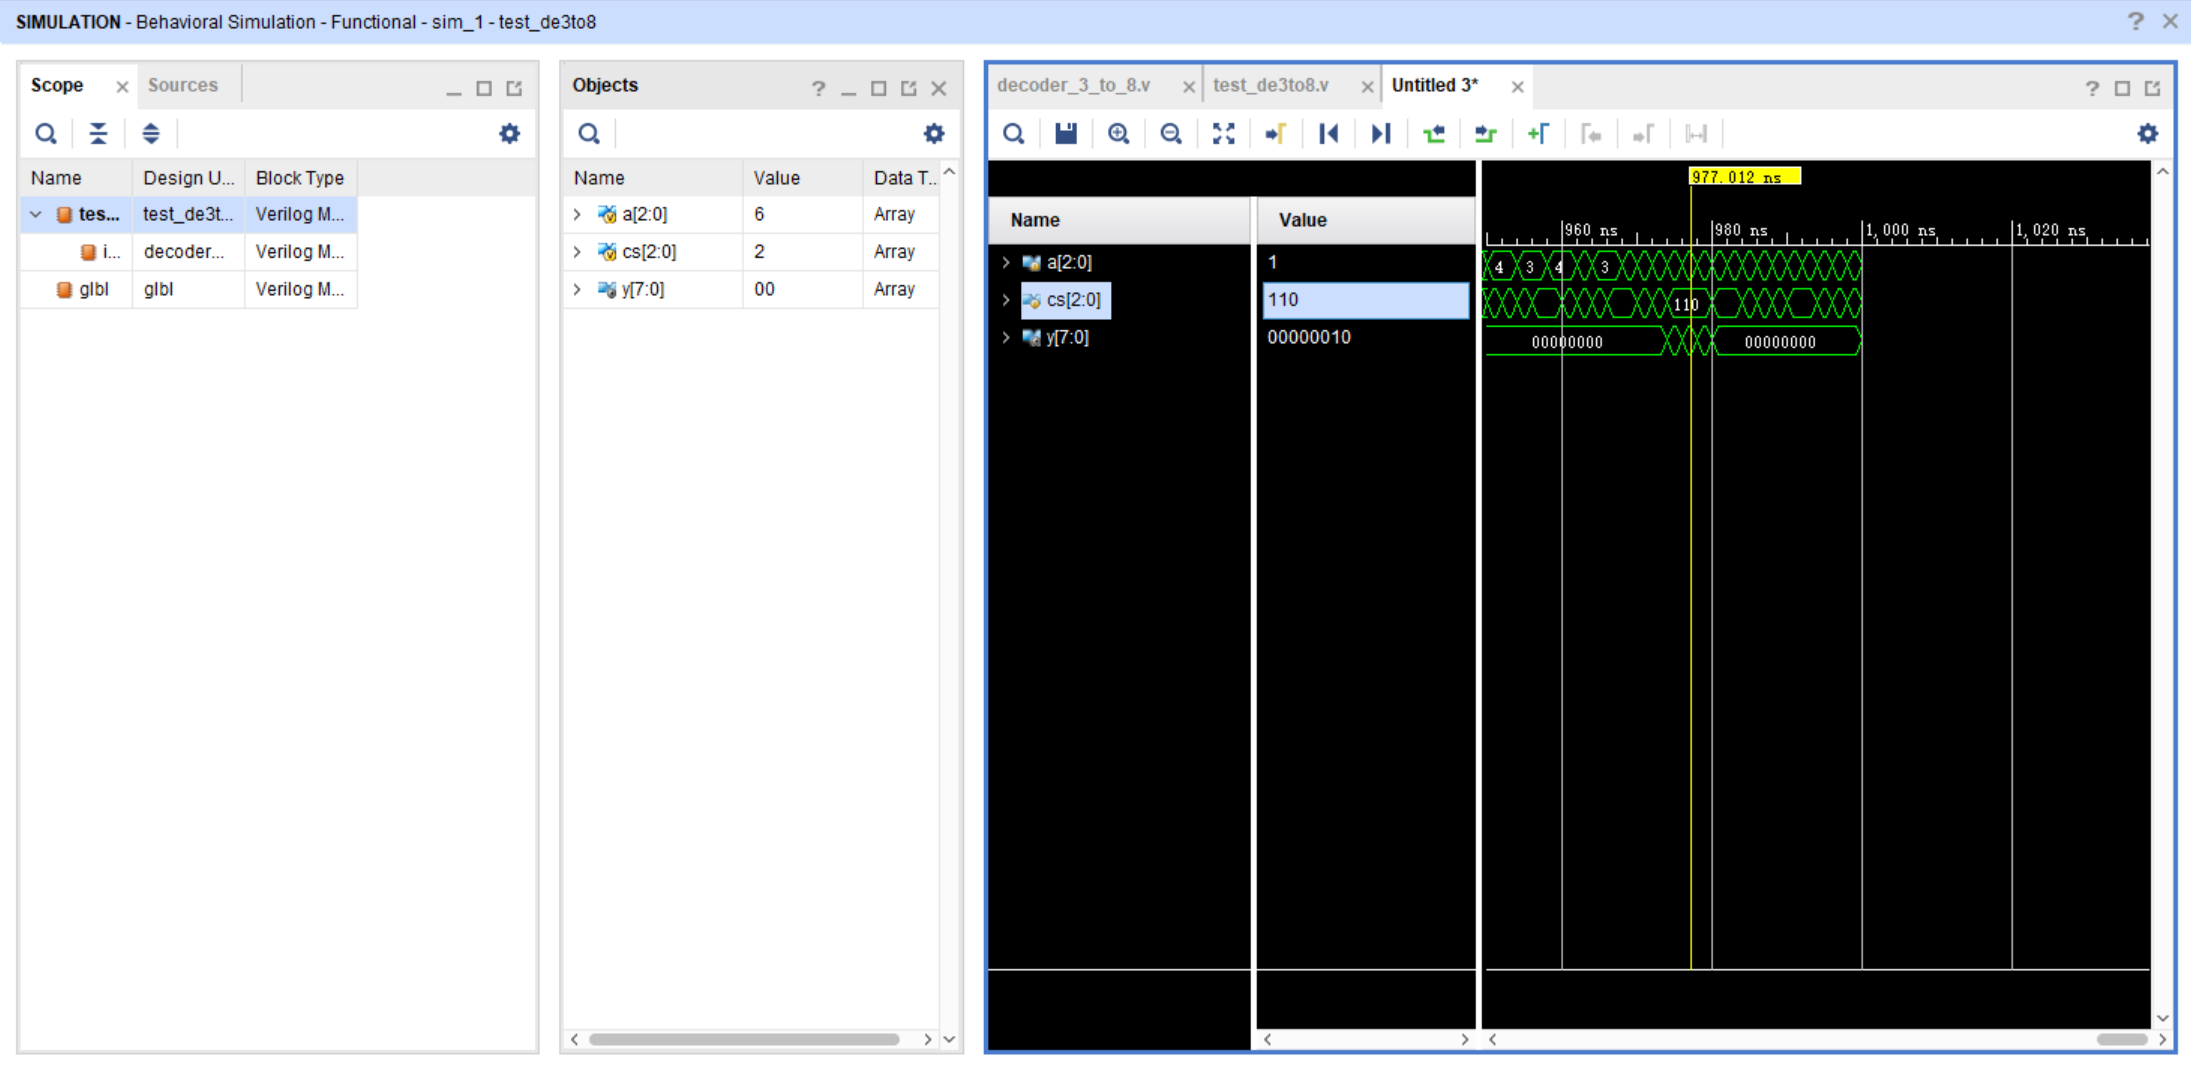
\includegraphics[width=500pt]{assets/image_decoder_3to8.png}
    \captionof{figure}{3--8译码器 Simulation 结果}
\end{center}

\section{实验总结}

通过本次实验,我熟悉了 Vivado 软件的操作过程和操作逻辑,进行了四位加法器的设计及其他电路的设计,验证了其功能。我得以深入理解组合逻辑电路的设计机制以及 Verilog 语言的使用,为日后更深入学习数字电路课程打好了基础。

\section{源代码}

\subsection{4位加法器}

File: add\_4.v
\begin{lstlisting}
`timescale 1ns / 1ps

module add_4(
    input [3:0] add_0,
    input [3:0] add_1,
    input c_in,
    output [3:0] out,
    output c_out
    );
    assign {c_out, out} = add_0 + add_1 + c_in;
endmodule
\end{lstlisting}

File: test\_add\_4.v
\begin{lstlisting}
`timescale 1ns / 1ps

module test_add_4();
    reg [3:0] in_0;
    reg [3:0] in_1;
    reg carry_in;
    wire [3:0] sum;
    wire carry_out;
    
    add_4 instance_add_4 (
        .add_0(in_0),
        .add_1(in_1),
        .c_in(carry_in),
        .out(sum),
        .c_out(carry_out)
    );
    
    initial begin
        in_0 = 4'b0001;
        in_1 = 4'b0000;
        carry_in = 1'b0;
    end
    
    always begin
        #2;
        in_0 = $random() % 16;
        in_1 = $random() % 16;
        carry_in = $random() % 2;
    end
endmodule
\end{lstlisting}

\subsection{全加器 (门电路版本)}

File: full\_adder.v
\begin{lstlisting}
`timescale 1ns / 1ps

module full_adder(
    input a,
    input b,
    input ci,
    output s,
    output co
    );
    assign s = (a ^ b) ^ ci;
    assign co = (a & b) | (a & ci) | (b & ci);
endmodule    
\end{lstlisting}

File: test\_full\_adder.v
\begin{lstlisting}
`timescale 1ns / 1ps

module test_full_adder();
    reg a, b, ci;
    wire s, co;
    
    full_adder inst_fa(
        .a(a),
        .b(b),
        .ci(ci),
        .s(s),
        .co(co)
    );
    
    initial begin
        a = 1'b0;
        b = 1'b0;
        ci = 1'b0;
    end
    
    always begin
        #2;
        a = $random() % 2;
        b = $random() % 2;
        ci = $random() % 2;
    end

endmodule
\end{lstlisting}

\subsection{3--8译码器 (高电平有效)}

File: decoder\_3to8.v
\begin{lstlisting}
`timescale 1ns / 1ps

module decoder_3_to_8(
    input [2:0] a,
    input [2:0] cs,
    output [7:0] y
    );
    
    reg [7:0] out;
    
    always @(*) begin
        case(a)
            3'b000: out = 8'b1;
            3'b001: out = 8'b10;
            3'b010: out = 8'b100;
            3'b011: out = 8'b1000;
            3'b100: out = 8'b10000;
            3'b101: out = 8'b100000;
            3'b110: out = 8'b1000000;
            3'b111: out = 8'b10000000;
        endcase
        
        if (cs != 3'b110) begin
            out= 8'b0;
        end
    end
    
    assign y = out;
endmodule    
\end{lstlisting}

File: test\_de3to8.v
\begin{lstlisting}
`timescale 1ns / 1ps

module test_de3to8();
    reg [2:0] a, cs;
    wire [7:0] y;

    decoder_3_to_8 inst_de3t8(
        .a(a),
        .cs(cs),
        .y(y)
    );
    
    initial begin
        a = 3'b0;
        cs = 3'b0;
    end
    
    always begin
        #2;
        a = $random() % 8;
        cs = $random() % 8;
    end
endmodule    
\end{lstlisting}

\end{document}